\section{Introduction}
Online news websites are now a common way of consuming news. These
websites are very helpful in publishing breaking news and help users
keep up to date with the latest developments. However, the
proliferation of these websites simply means that we are drowning in
more news than we know what to do with. Specific news stories that we
would like to follow over days or weeks may be buried among more
current or recent news. Navigating through a maze of articles looking
for ones of interest is a non-trivial task.  

Current news websites do not do much to help users trace the origin of
these stories, nor how they overlap with each other. Most of them
still ``look'' like news papers with a bunch of articles laid out on
the web-page, with a few additional features in the form of ``Related
News'' and ``Recommended News'' links. A reader trying to
contextualize a particular article can follow some of these links but
the context provided by these features is shallow and tracing the
development of the story with its various aspects is not much easier
than it was in the days of paper-based news media. The news corpus is
available in electronic form, carefully archived by all news
organizations. There have been some recent efforts by the research
community that attempt to extract individual strands of a stories
development from the corpus~\cite{shahaf@kdd2010} or present
interacting strands in a mesh-like
structure~\cite{shahaf@www2012}. Still others use graph-like
abstractions, just like we do, to approach the limited problem of
detecting a news item that represents the development of a news
story~\cite{subasic-icdm:2008,subasic-ida:2013}. What remains missing
is the structural framework required to process it into a form that
would make it possible for a user to elaborate the many contexts
behind a single news story, some stretching years into the past, some
just a few days. 

To make this concrete let us consider the unfortunate gang-rape
incident that took place in Delhi in December 2012. Since the day this
crime was first reported by the media, it grew into a complex news
story, talking about related rape cases of the past, the reactions of
various sections of the society (politicians, activists, human rights
organizations, etc), the health of the victim up to her tragic death,
the investigation carried out by the law enforcement authorities and
the judicial proceedings against the offenders once they were
caught. Different users may want to focus on different aspects of this
story. For eg., consider a graph of news articles around this story
shown in Figure~\ref{fig:context-adding-graph-gang-rape-1}.  We see
three of the many possible contexts that can be followed and utilized
by a user to better understand the overall picture. We allow the user
to express her intent to follow a particular context (either ``the
reactions of Politicians'' or ``the victim's condition'' or ``the
Police investigations'') and understand the story with that
context. This results in a view that is personalized for a particular
user, since she is free to choose the context(s) that help her follow
the story. We call this notion \emph{Personalized Flexible Context
  Extraction}. This notion is an extremely natural approach that a news
consumer, whether an expert commentator or a lay person, might want to
employ as a crucial subtask in the process of news consumption. We
believe that it is possible to realize this notion given the
development in information extraction techniques that has taken place
in the last few years. However this realization requires the
specification and implementation of a  framework for
(pre)processing and structuring the news corpus in such a way that it
can easily serve information needs that cannot always be forseen when
the news emerges.

\begin{figure}[ht]
\caption{How multiple contexts are added to a single story}
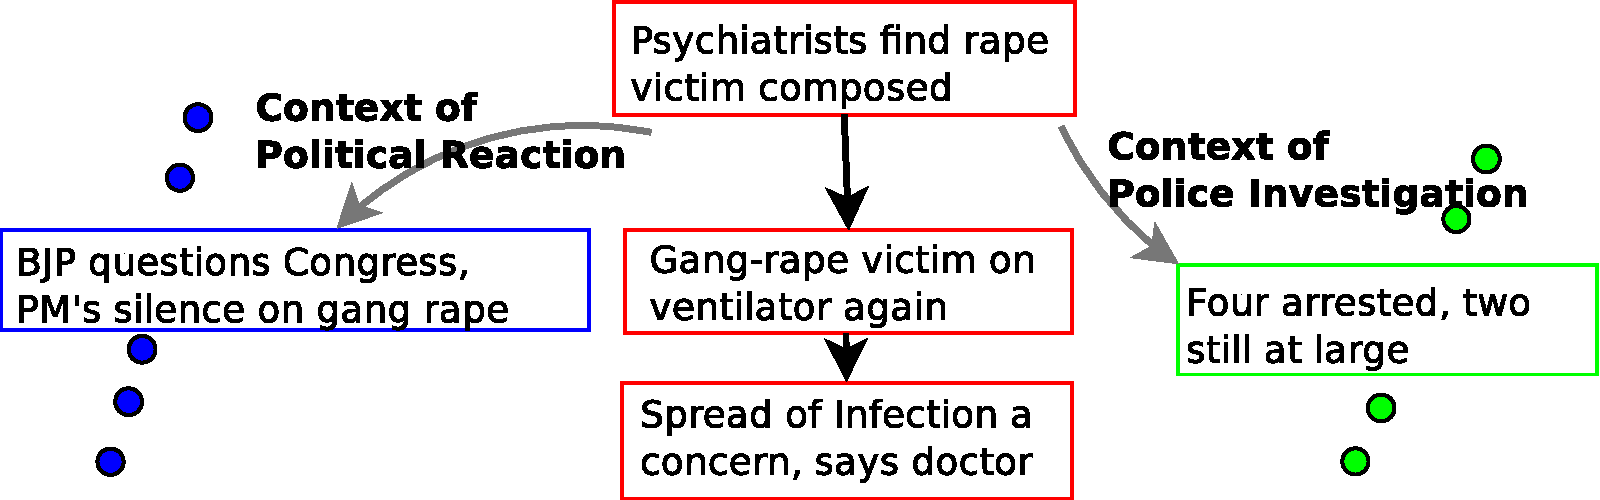
\includegraphics[scale=0.31]{figures/graph-3.pdf}
\label{fig:context-adding-graph-gang-rape-1}
\end{figure}


%What we want to do about it -- this paragraph is pretty weak
Our attempt in this paper is to provide such a framework and show that
it can be used in a flexible way by a user to fulfill his or her need
to contextualize what he or she is reading in the news.  Building on
the work of~\cite{choudhary@ecir2008} that models news corpora as a
time-evolving graph by linking related news articles, we provide a
query mechanism that organizes this structure by topics of interest
and important actors, and presents the development of a story on a
timeline. The user can now interact with the result by filtering
articles based on topic, entities, time, or a combination of all
three. For example, Figure~\ref{fig:complete-tool-screenshot} shows
the timeline of the recent rape case incidents reported from India.

An important aspect of our work that represents a completely different
approach from the prominent attempts at news corpus processing and
extraction in the literature is that we take an offline approach
i.e. we view the news corpus as an evolving entity that is streaming
past us. We store it in a structured way such that it can be browsed
and, importantly, {\em different kinds of contexts can be extracted
  from it by users with different approaches to the same news
  stories}. This represents a break in thinking from those approaches
that take the entire news corpus as their input and either produce an
output which {\em is} the story~\cite{shahaf@kdd2010,shahaf@www2012}
or produce some output based on a pre-existing notion of what is the
story~\cite{subasic-icdm:2008,subasic-ida:2013}. We allow the user to
build the story. Apart from providing lower flexibility to the user,
in our opinion, these other approaches are fundamentally not-scalable
since every time an information need arises a set of expensive
computations has to be done. Our approach can be thought of as a
data-structuring approach: We preprocess the data to make news
browsing and user-led context discovery an easier and computationally
feasible process.

%Contributions
In summary, our contributions are as follows:
\squishlist
\item We build on a graph-based framework (\cite{choudhary@ecir2008}) to represent articles in a news corpus and make it query-able. 
\item We propose metrics to capture utility of a news article to understand a news story in terms of the coherent context provided by it.
\item We propose an efficient graph-based algorithm to find useful contexts around a news story that help to get the bigger picture.
\item We provide an interactive interface to users which is easy to use, and helps in tracking the evolution of the story and zooming
  to specific parts of interest.
\item We report on the results of a thorough evaluation of our system and show that our system compares well with existing ones.
\squishend

\textbf{Organization:} The rest of the paper is organized as
follows. We first summarize the related work that has addressed the
problem of news corpus mining, categorizing it under various threads
(Section~\ref{sec:related}). We then formally state our definition of
a personalized flexible context extracting news browsing tool,
describing the basic features of such a tool and our approach to
building such a tool based on the news graphs
of~\cite{choudhary@ecir2008} (Section~\ref{sec:newsgraph}).  In
particular, we introduce the notion and importance of \emph{context}
of this news graph, and describe how these contexts can be extracted.
Next, we give a detailed block-by-block description of our system
(Section~\ref{sec:block}). We then present results from various
evaluation experiments conducted on our news browsing system
(Section~\ref{sec:eval}). Finally, we conclude with some
observations and future scope (Section~\ref{sec:conclusions}).
